\chapter*{List of Appendices}

\begin{enumerate}
\item Obrázek \ref{rrs_ML}
\item Obrázek \ref{rpoB_ML}
\item Obrázek \ref{rpoD_ML}
%\item \hyperlink{SPARC.1}{Titulní strana sborníku SPARC 2016}
%\item \hyperlink{SPARC.55}{Abstrakt z příspěvku v rámci SPARC 2016}
%\item \hyperlink{fenotyp.1}{Shluková analýza fenotypu}
%\item \hyperlink{ordination.1}{Ordinační analýza fenotypu}
%\item \hyperlink{genotyp.1}{Shluková analýza genotypu}
\end{enumerate}

\addcontentsline{toc}{chapter}{Appendix}
%\pageref{mypage}
%\hyperlink{fenotyp.1}{Dendrogram biochemie}
%\includepdf[link, linkname=fenotyp, pages=1, landscape, angle=270, fitpaper]{text_prace/Pictures/anal_vse_ward_jacc_colXYZA.pdf}

%\includepdf[link, linkname=ordination, pages=1, landscape, fitpaper]{text_prace/Pictures/anal_vse_PoCA_jaccard_big1.pdf}

%\includepdf[link, linkname=genotyp, pages=1, landscape, angle=270, fitpaper]{text_prace/Pictures/RPearson-reduction_XYZA_colFULL1.pdf}
\begin{figure}[h!!!]
  \centering
  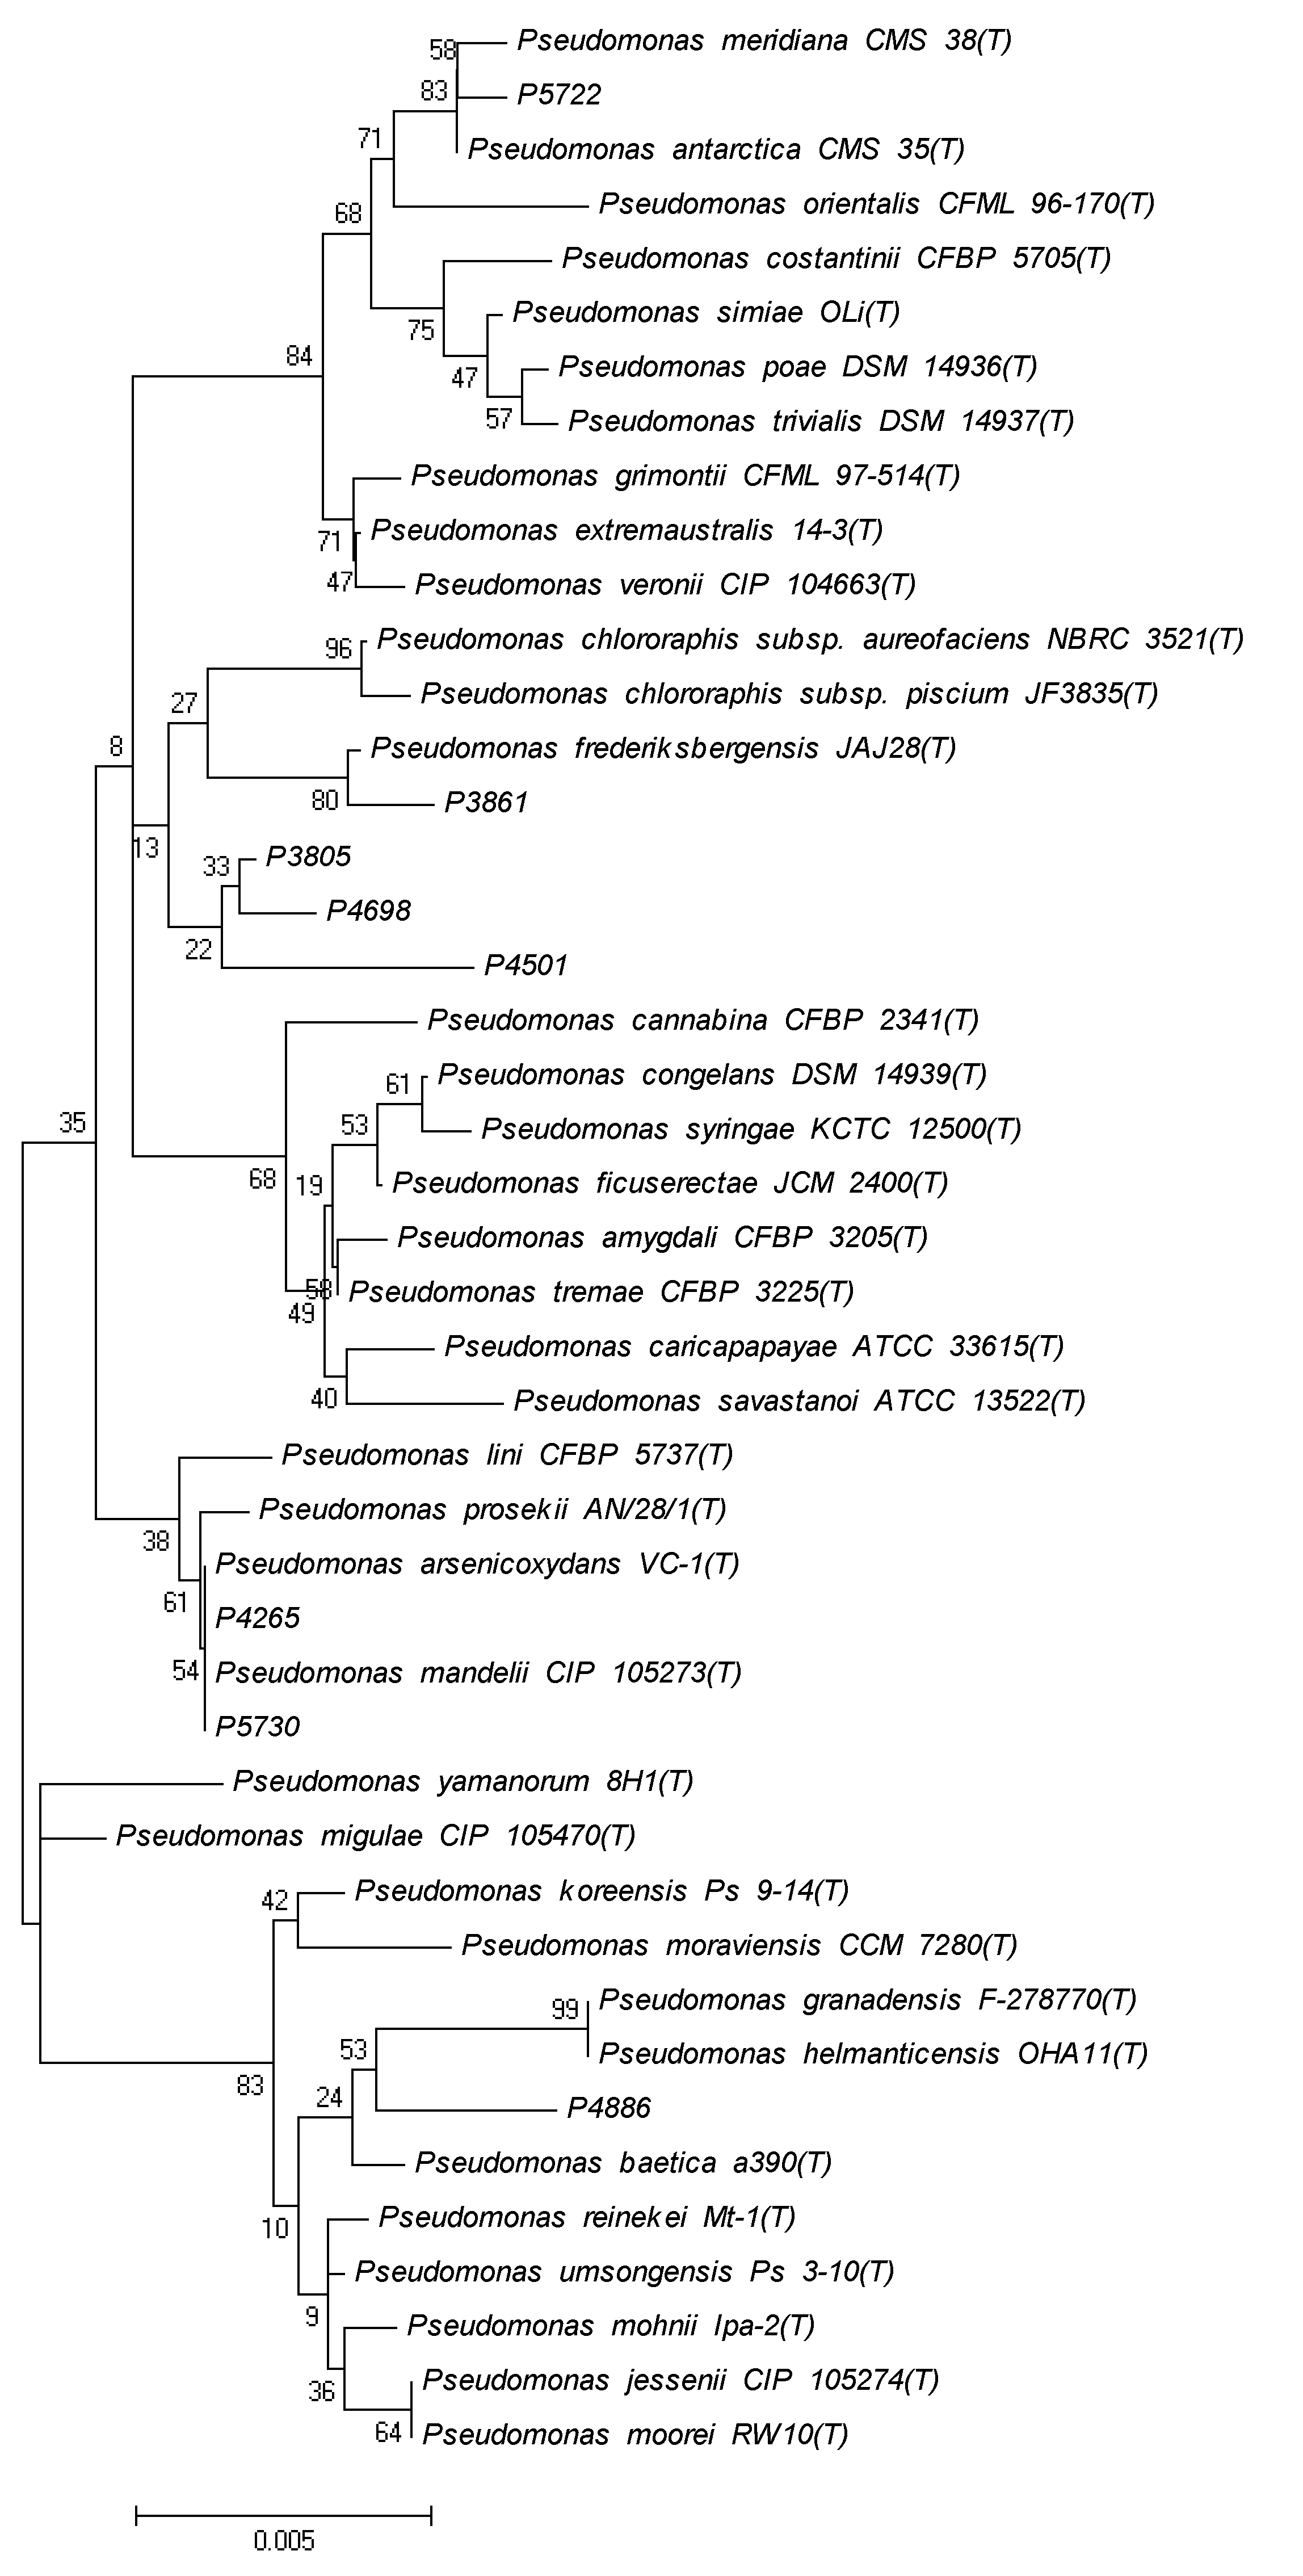
\includegraphics[scale=0.50]{text/Pictures/160508_16S_ML_clustalW_Bootstrap-consensus.png}
	\caption{Fylogenetický strom na základě analýzy genu \tax{rrs} dle metody Maximum-likelihood}
	\label{rrs_ML}
\end{figure}
\pagebreak

\begin{figure}[h!!!]
  \centering
  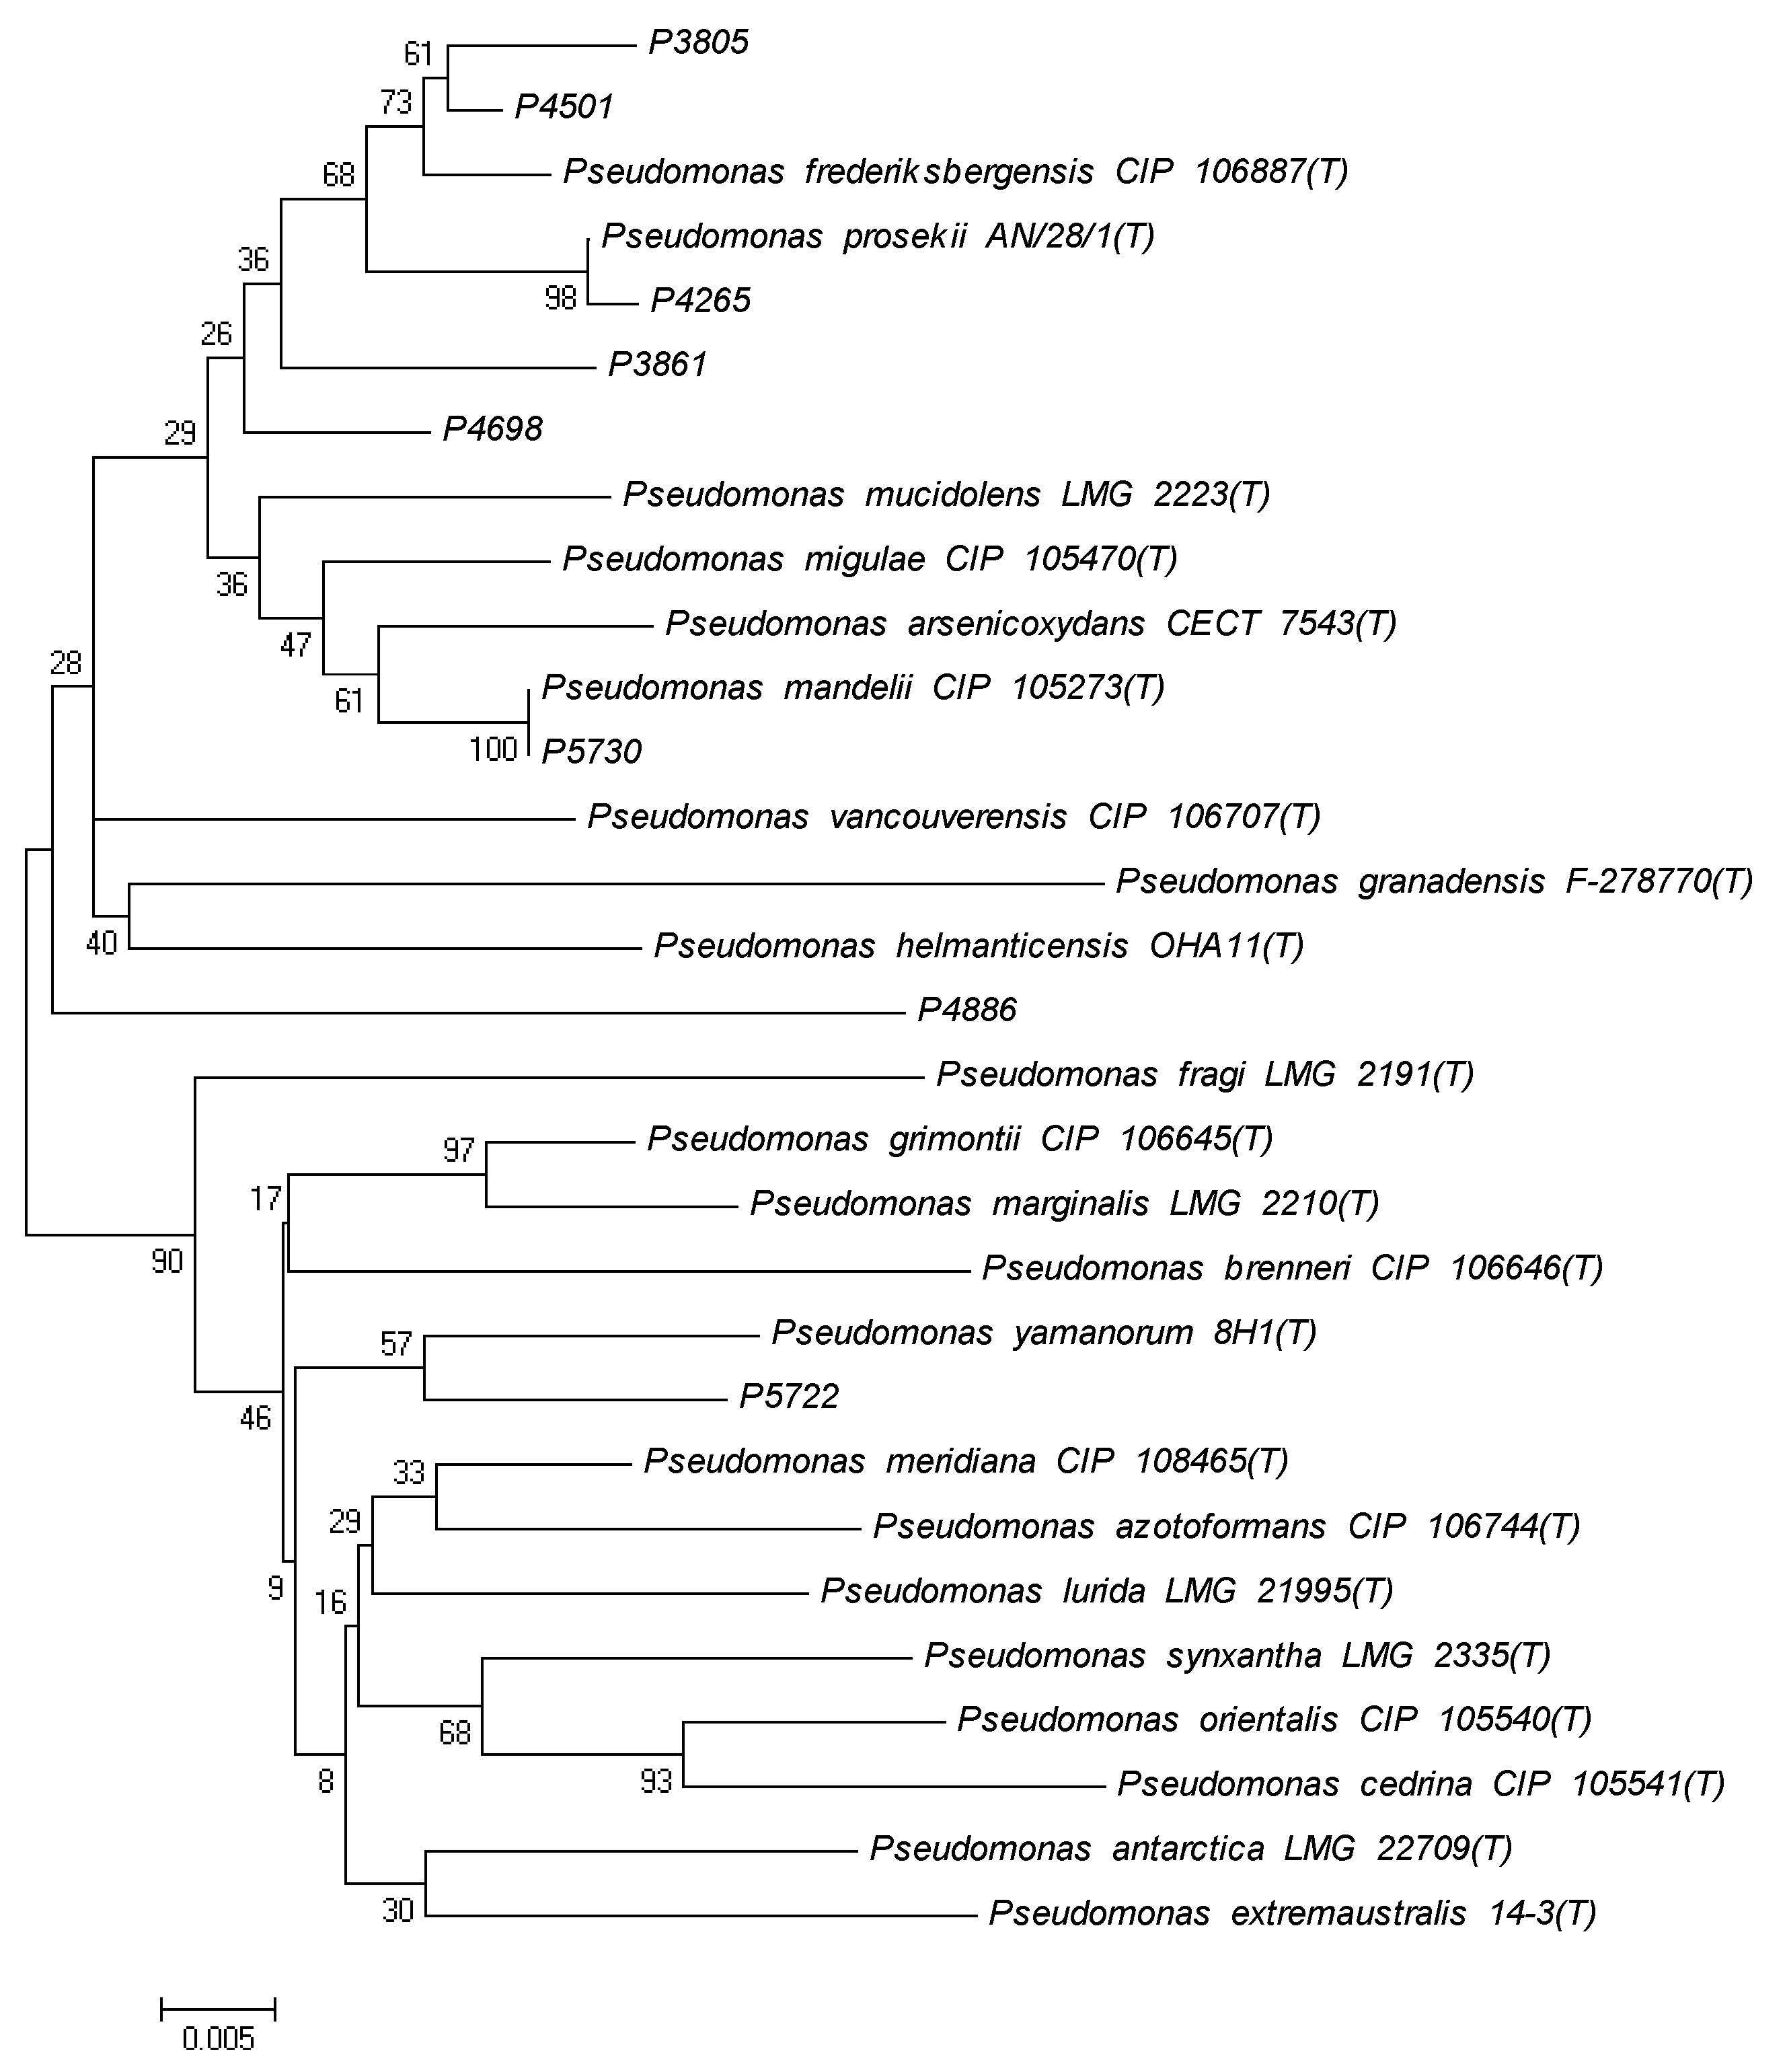
\includegraphics[scale=0.50]{text/Pictures/160508_rpoB_multifasta_doplnek_ML_clustalW_Bootstrap-consensus.png}
	\caption{Fylogenetický strom na základě analýzy genu \tax{rpoB} dle metody Maximum-likelihood}
	\label{rpoB_ML}
\end{figure}
\pagebreak

\begin{figure}[h!!!]
  \centering
  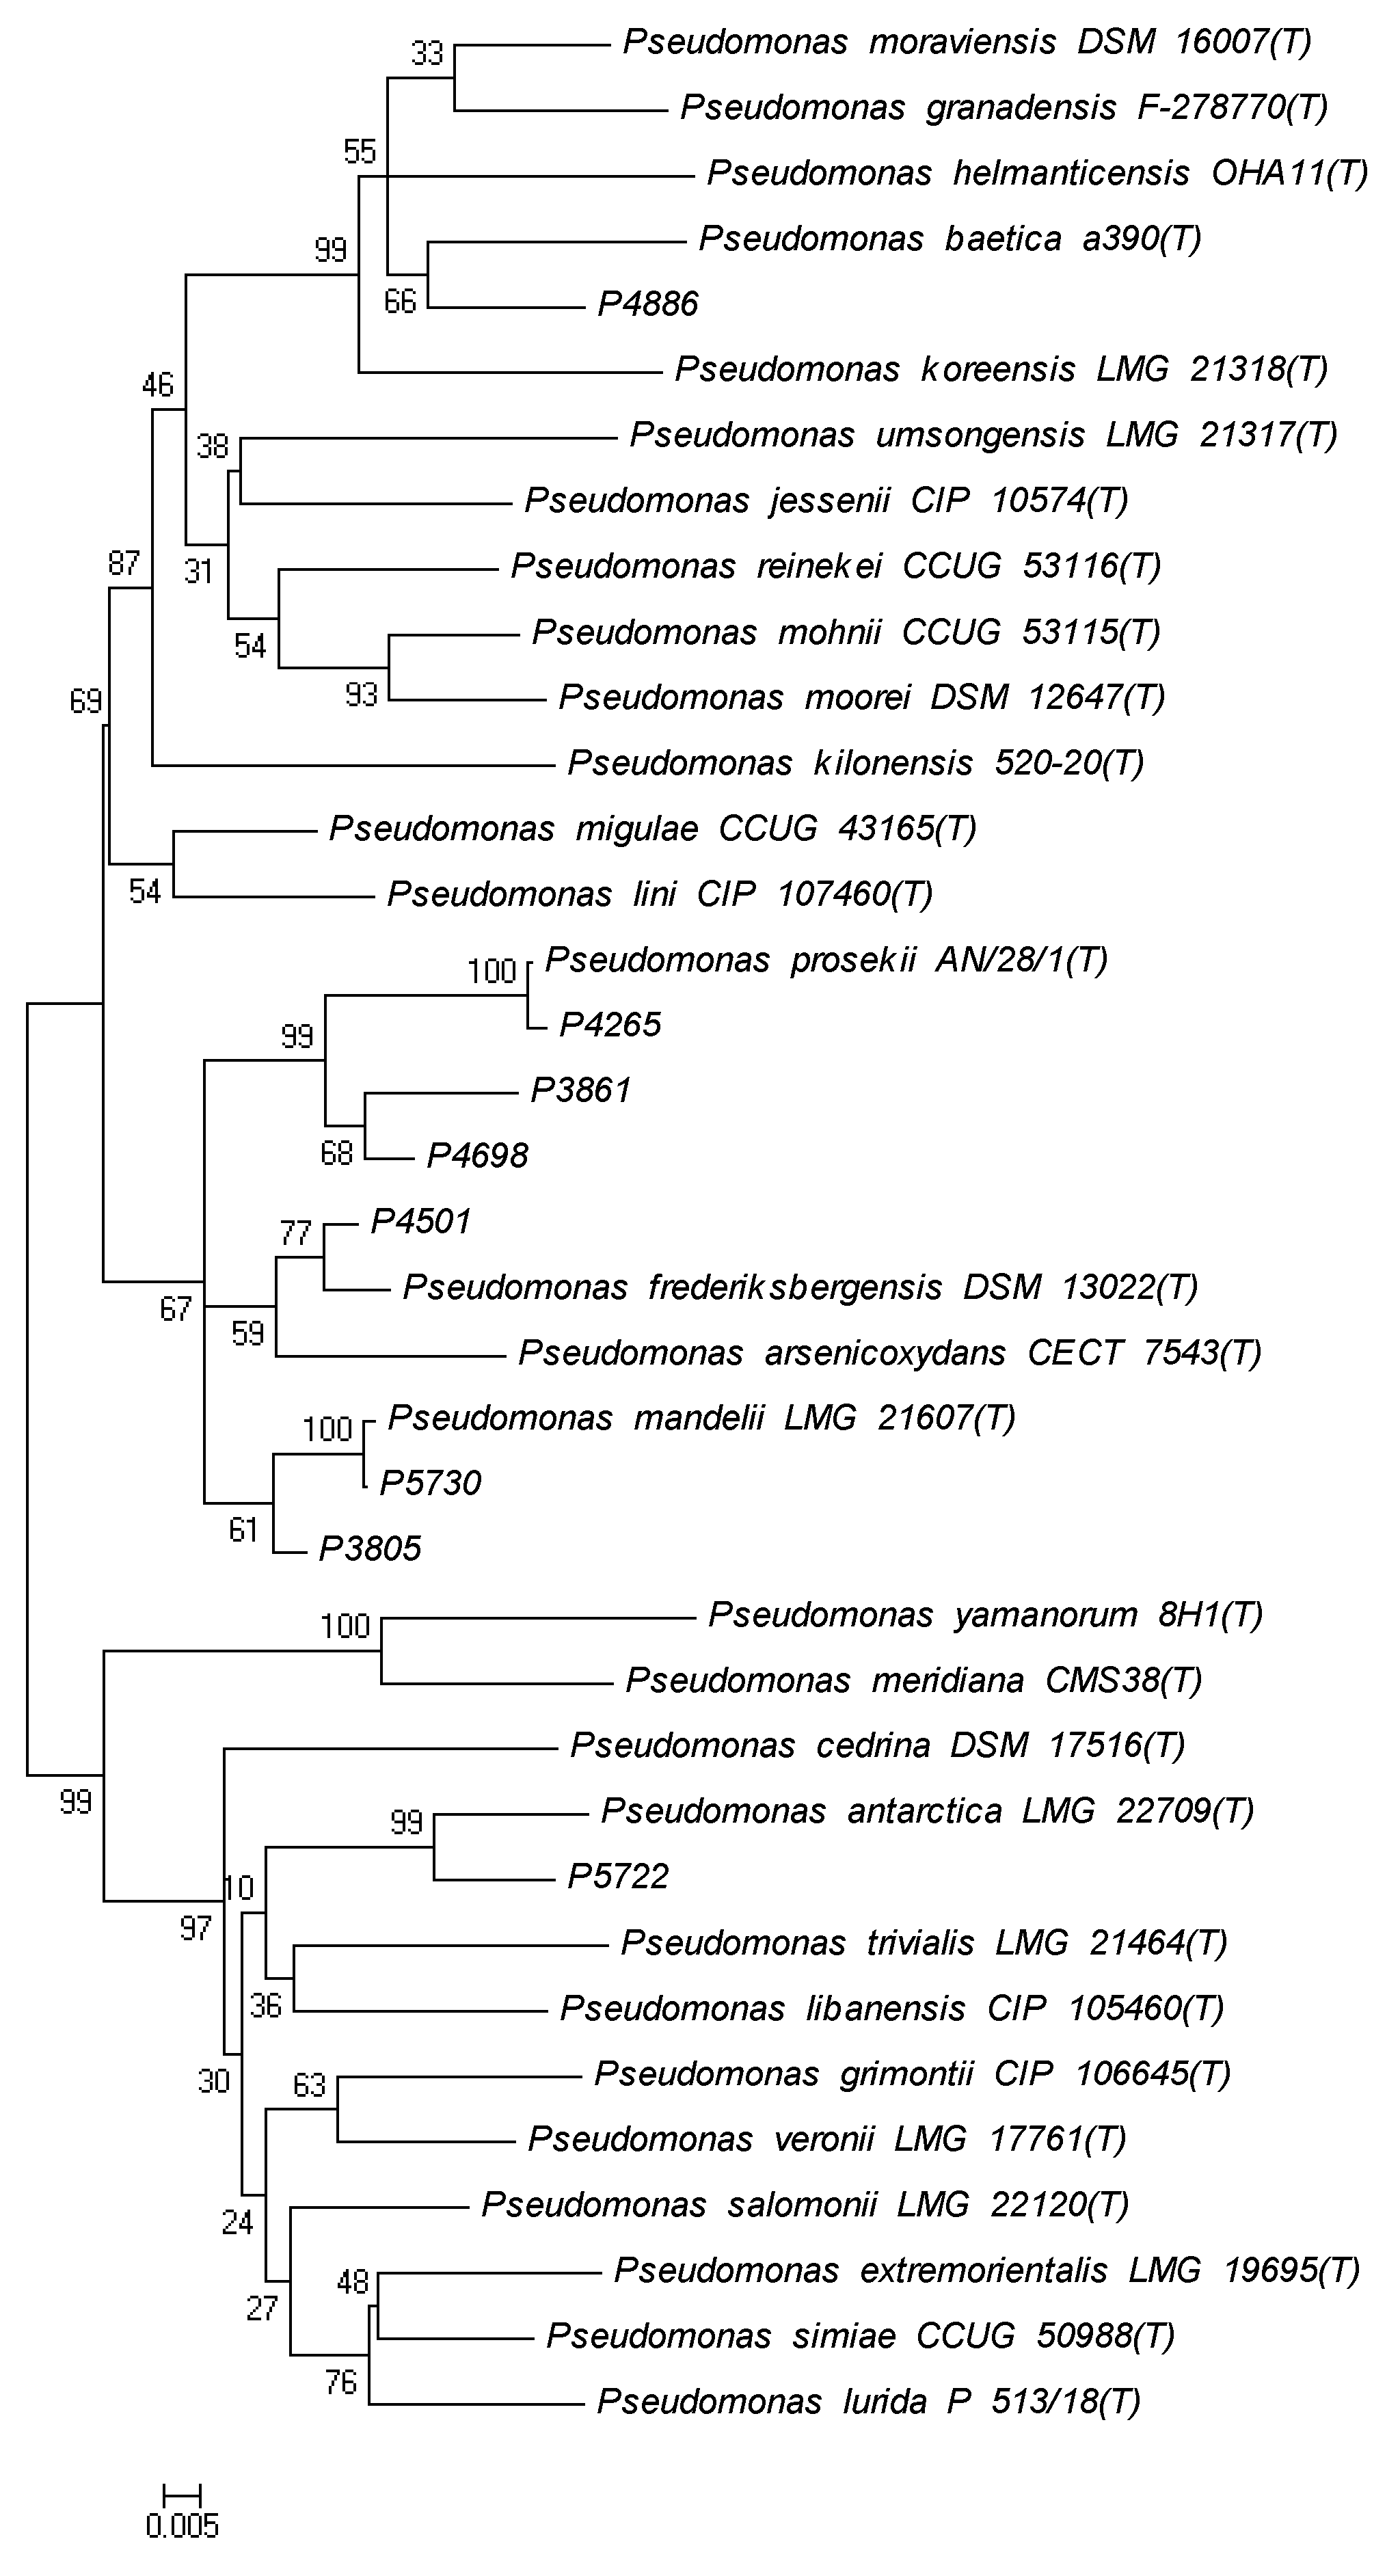
\includegraphics[scale=0.50]{text/Pictures/160508_rpoD_multifasta_doplnek_ML_clustalW_Bootstrap-consensus.png}
	\caption{Fylogenetický strom na základě analýzy genu \tax{rpoD} dle metody Maximum-likelihood}
	\label{rpoD_ML}
\end{figure}
\clearpage

%\includepdf[link, linkname=SPARC, pages=1, landscape, fitpaper]{text/Pictures/Sbornik-SPARC2016.pdf}

%\includepdf[link, linkname=SPARC, pages=55, landscape, fitpaper]{text/Pictures/Sbornik-SPARC2016.pdf}

%Here is a \hyperlink{anal_vse_ward_jacc_color3.pdf.19}{hyperlink to page 19} of anal_vse_ward_jacc_color3.pdf.

%\medskip

%%%%%%%%%%%%%%%%%%%%%%%%%%%%%%%%%%%%
%%%%%%%%% GENERUJ TEXT %%%%%%%%%%%%%
%%%%%%%%%%%%%%%%%%%%%%%%%%%%%%%%%%%%

\cleardoublepage
